As we have seen from the Aquapod, the addition of the water domain capability greatly expanded the opportunities for environmental monitoring relative to the Adelopod. 

% Expansion to operational environment 
The acqueous ability allowed a whole new set of sensing opportunities and greatly expanded the nature of the environmental monitoring tasks that could be undertaken. 

% Navigational expansion 
Analogously, terrains that were once inaccessible to a terrestrial platform, such as lakes, puddles, and streams were now traversable. Furthermore, unfavorable obstacles such as mud, snow were now also available. 



As seen with the land-water robot concept \ref{sec:aquapod_v1}, the addition of the water domain greatly expanded the capabilities for environmental monitoring 
Leveraging fundamental design elements of the Aquapod, such as the waterproof hull and buoyancy control unit, the amphibious Screwdrive actuator for land and water locomotion, and a quad-rotor configuration for flight, the Omnibot is proposed as a multi-domain robotic platform for environmental monitoring. While there are robots capable of amphibious (land-water), air-ground, and air water locomotion, to the author's knowledge, the Omnibot would be the first to navigate all three environments. 

The MUWA \cite{Kawasaki2013}, Fig~\ref{fig:muwa}, consists of a traditional quad-rotor layout enveloped by a dual styrofoam rings on its periphery. As would be expected, the robot flies as is typical of a quadcopter. When on land, it is able to use differential thrust from its variable pitch propellers to stand itself up on its side and roll on the outer rings as a mono-wheel. Furthermore, the positively buoyant external rings enable the robot to float on the surface of the water and the actuators provide ability to move about in a limited fashion. That being said, the robot is not claimed to be capable of underwater operation, neither in construction nor locomotion.  


\begin{figure}[!ht]
  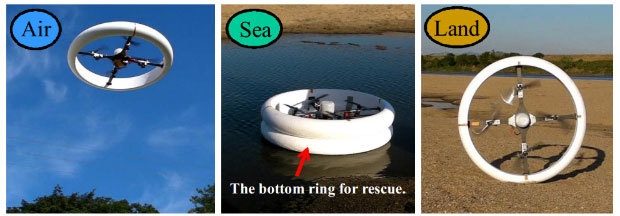
\includegraphics[width=\linewidth]{images/muwa.jpg}
  \caption{The MUWA model (courtesy of \cite{Kawasaki2013})}
  \label{fig:muwa}
\end{figure}

\subsubsection{Design Contraints}

Operation in the three domains is more than the combination of parts as constraints for one domain are often at odds with another domain's contraints. Some contraint conflicts are obvious, such as the minimum necessary weight to enable land and water operation versus flight performance. Other constraints, such as approximately neutral buoyancy, are more nuanced, since weight minimization would be favorable for flight but weight may need to be added in order to match that required my the minimum volume displaced by the platform. 

Design constraints are categorized into locomotive and structural. Locomotive covers the means by which the Omnibot is to move itself through a given domain and structural pertains to the physical properties of the platform's structure.

\emph{Transitions}

\subsubsection{Locomotion Design}

Central to the functionality and usability of a mobile robotic platform is the methods by which it moves itself through the environment it is in. The locomotive system is a fundamental choice as it often is the most energy consuming aspect. Actuator choice often determines the type of battery to be used and affects the run time of the robot. Furthermore, the type of terrain and navigational solutions are determined by the ability of the locomotive system. 


The Screwdrive was chosen for the Omnibot due to its light weight, simplicity, robustness, and amphibious nature.  In terms of both weight and volume the Screwdrive is favorable, however the key enabling feature is its amphibious function as it forgoes separate systems for land and water locomotion, thereby minimizing weight, volume, and complexity. 

A variable-speed quad-rotor system was chosen for flight due to its stability, vertical-take-off-and-lift (VTOL), payload capacity, and hovering capabilities. 

% Thrusters 
A quad-copter design was chosen based on its ability to provide the amount of thrust necessary to lift the platform, its ability to offer vertical-take-off-and-lift (VTOL), but most importantly because it allows effective air to ground and water transitions and vice versa, without impeding the other modes or transitions. 

The VTOL capabilities and controllability allow the robot to land carefully atop the screwdrive subsystem. Similarly, when transitioning from water the Omnibot was designed in such a way that the propellers are near the top of the robot and able to fly. Fixed-wing alternatives would have placed additional and incompatible restrictions on weight, size, and other variables all while increasing the size. 


\subsubsection{Mechanical Design}

Most of the OmniBot's electronic parts are enclosed in a waterproof transparent sphere, making it easy to take off and land due to less friction. On the other hand, the transparency allows for cameras to be added inside as well. 

A removable payload “disc” around the globe can be used to extend the capabilities of the robot in various important ways. Different sensor suites will be mounted on the disk in such a way to allow easy deployment of many OmniBots with different payloads.

\subsubsection{Weight and Cost}

By integrating multiple mechanisms together, we have built a prototype, the weight of which is around 1.4 kg, and the cost is less than \$1,000 USDs. Therefore, it is cost-effective to deploy in different environments to test its capabilities.

\subsubsection{Density}

The buoyancy control unit works by ingesting water such as is the case in the Aquapod section \ref{sec:aquapod_v1} and altering the robot's mass. Since the bladder is contained within a fixed volume, the density changes:

$$ \rho_{omnibot} = (mass_{omnibot}+mass_{bladder})/volume_{omnibot} $$ 

When the mass of the ingested media is enough to alter the OmniBot's density above that of the media it is contained in, it sinks. Reversing this process leads to the robot floating upwards towards the surface. 

$$ \rho_{omnibot} > \rho_{water} $$
$$ \frac{\rho_{omnibot}}{\rho_{water} } > 1 $$
$$ \rho_{water} = 1000 \frac{kg}{m^3} = 1 \frac{g}{cm^3} $$ 

\subsubsection{Sealing}
The main seal of the OmniBot consists of a face type seal employed between the two flanged hemispheres that comprise the main body of the robot. The hull halves squeeze an O-ring that is contained within a gland. This O-ring together with the gland provide protection for more than the equivalent of 5 meters of internal and external pressure. 

The numerous connections for the thrusters and screwdrive motors on the exterior of the robot are made through cable penetrators which also employ an elastomer to seal the interface where the surface is breached while allowing cables through. These are also removable by removing a nut, which is necessary for the maintainance of a field robot. 

\subsubsection{Electronics and Software}

The Omnibot electronics consist of an integration of COTS parts. Flight is achieved by using brushless electronic speed controllers that control the lightweight yet powerful T-Motor motors coupled to the rotors. The Pixhawk 4 platform \cite{pixhawkadmin_introducing_2018} and the PX4 flight stack \cite{noauthor_open_nodate} provide the flight control. Two brushed motors power the screwdrive and one additional motor is used for the buoyancy control unit, these three are controlled with brushed motor electronic speed controllers. 

The PX4 stack is modified to allow powering all the additional actuators and to allow switching between different operational modes or states: UAV, UGV, USV, and UUV. 


The overall state machine model of the system is composed of an UAV, UGV, USV, and UUV, driving distinct propelling mechanisms according to their respective control algorithms.

\subsubsection{Experiments and Results}
\label{experiments_omnibot}

With the constructed model, we firstly tested it in each individual setting, then we verified that it can switch between different modes to adapt to different scenarios, as detailed below.

\subsubsection{In the Air}

Equipped with four light yet powerful rotors, OmniBot is able to fly up as a common quad-rotor drone. In Figure \ref{fig:omni_flight}, the OmniBot is taking off. 


\begin{figure}
  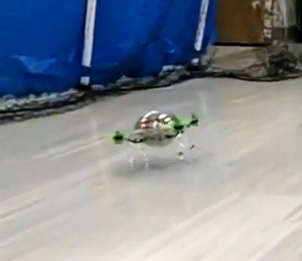
\includegraphics[width=\linewidth]{images/omnibot/omnibot_flight_2.PNG}
  \caption{The OmniBot is taking off}
  \label{fig:omni_flight}
\end{figure}

\subsubsection{On the Ground}

As seen from Figure \ref{fig:omnibot} when put on the ground, the robot can move around using two screw drives, which are especially suitable for exploration of sandy or muddy areas.

\begin{figure}
  \includegraphics[width=\linewidth]{images/omnibot/omnibot_isoview.JPG}
  \caption{The Omnibot on the ground.}
  \label{fig:omnibot}
\end{figure}

\subsubsection{On the Water Surface}

As seen from Figure \ref{fig:omni_surface_top}, since the overall density of the OmniBot is less than the water, it can float in the water and move around thanks to the screwdrive mechanism.

\begin{figure}
  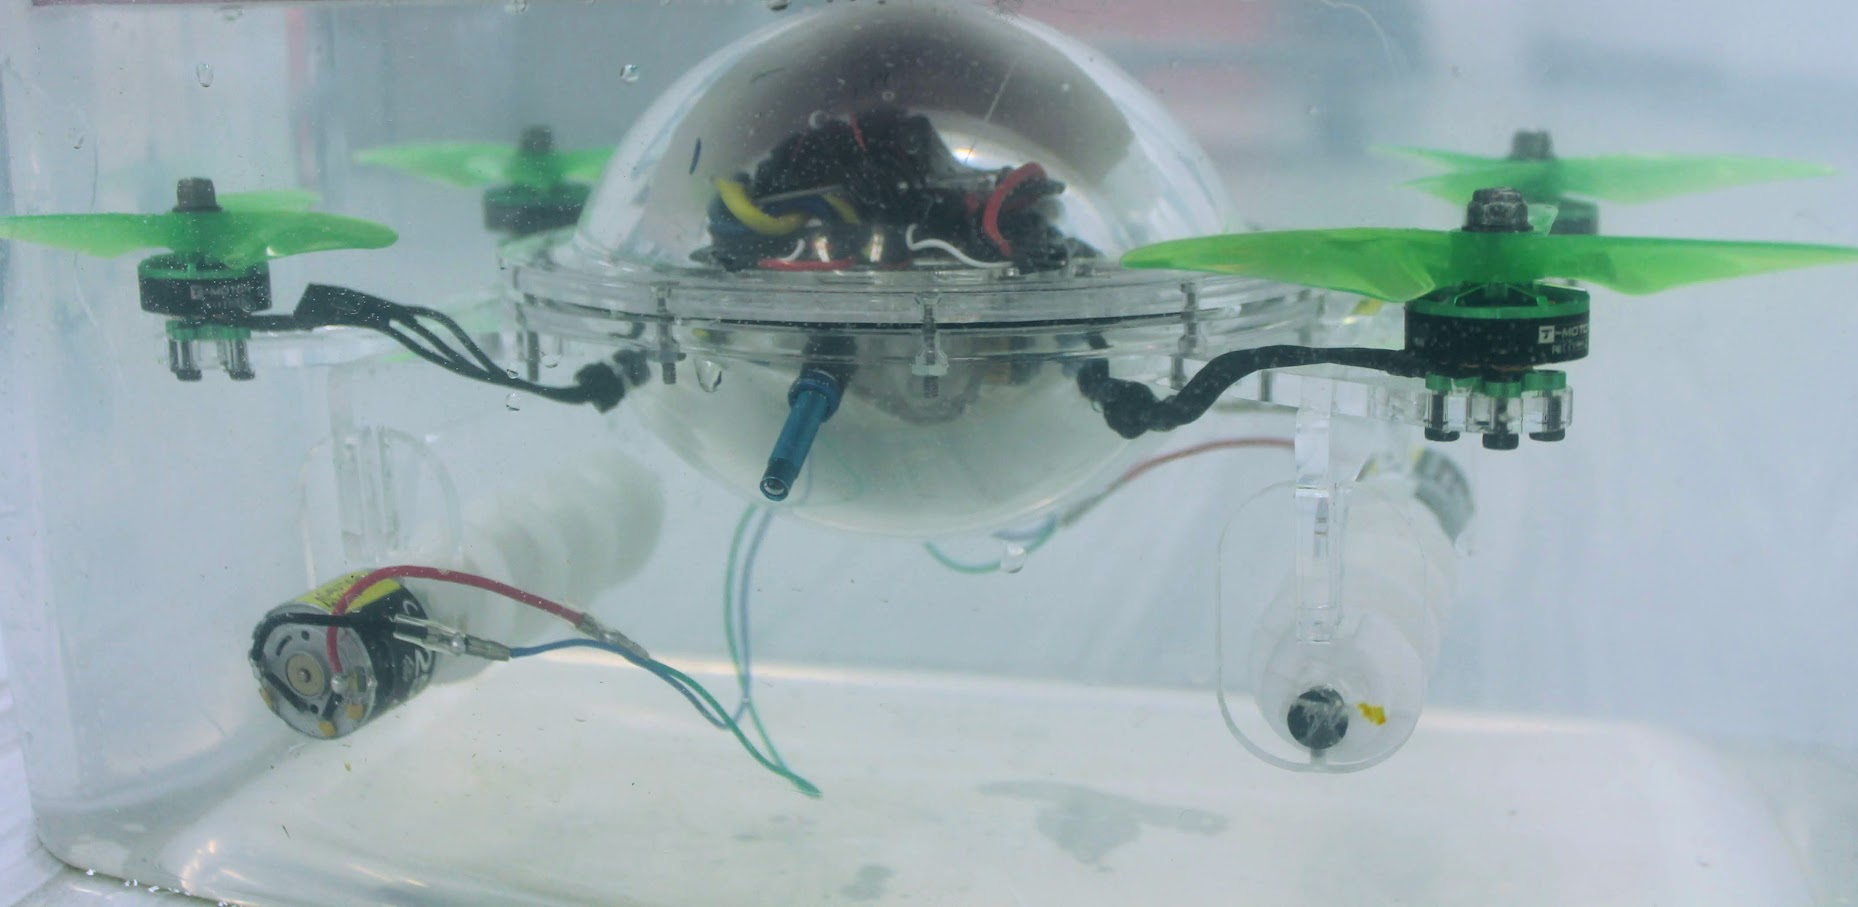
\includegraphics[width=\linewidth]{images/omnibot/omnibot_submerged_back.JPG}
  \caption{The Omnibot under water.}
  \label{fig:omnibot_submerge}
\end{figure}

\subsubsection{Under the Water}

By pumping water into the shell, the well-sealed OmniBot can dive into the water as well, as can be seen in Figure \ref{fig:omnibot_submerge}.

\begin{figure}
  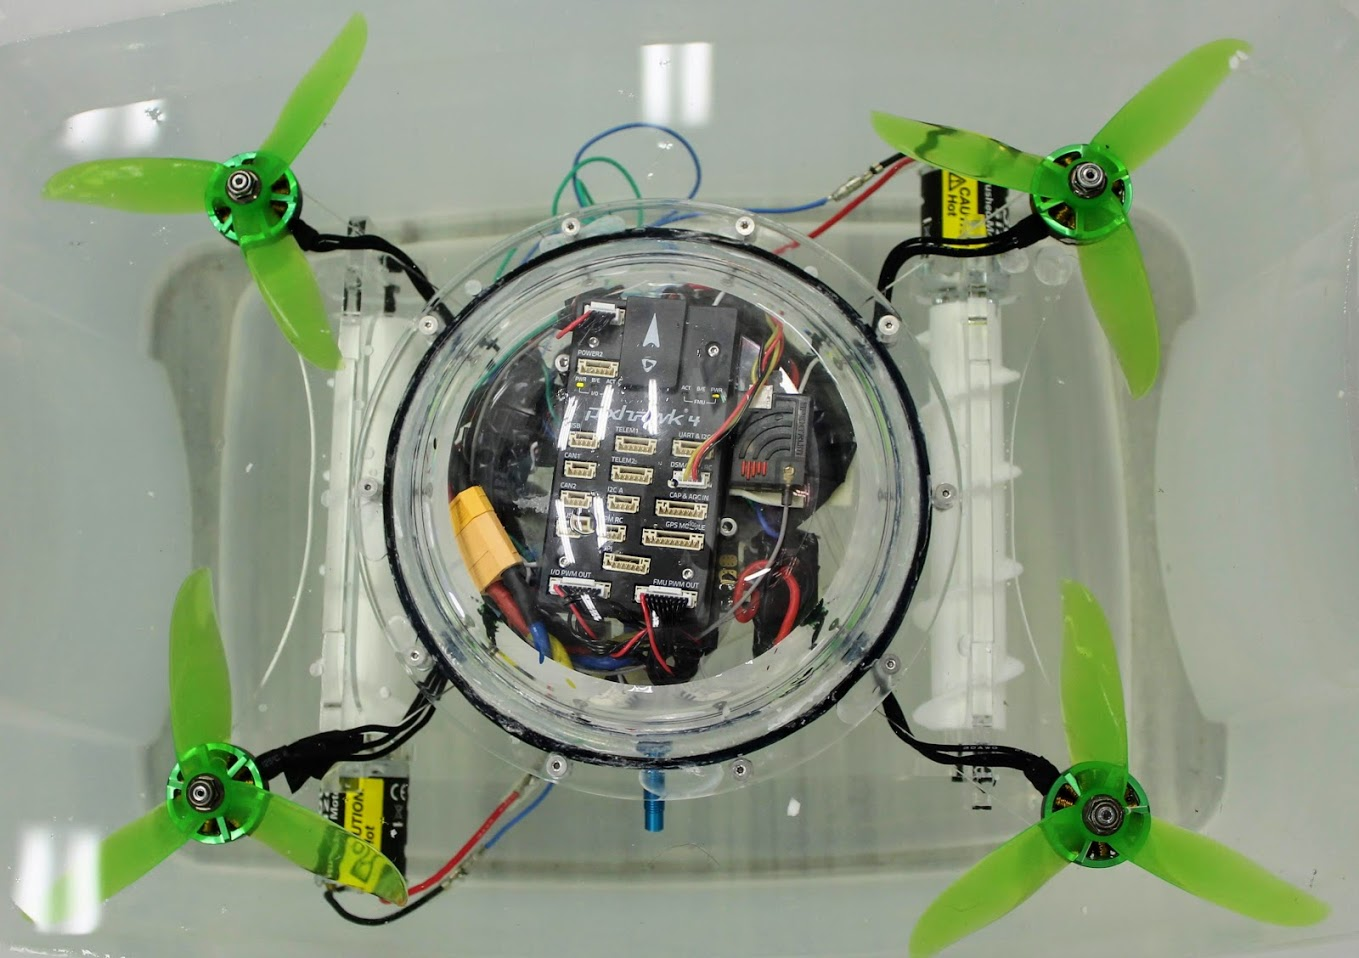
\includegraphics[width=\linewidth]{images/omnibot/omnibot_surface_top.JPG}
  \caption{The OmniBot is under water}
  \label{fig:omni_surface_top}
\end{figure}

\subsubsection{Transitions Between Varying Modes}

After testing the OmniBot in each individual environment, we also verified its capability of adapting from one kind of active area to another. A detailed video has been uploaded to demonstrate transitions between air, land, and water. 





%kk\subsubsection{On the Water Surface}
%Omnibot background ------------------------------------------------------------------------------------
%On the other hand, there have also emerged a handful of systems that can perform tasks in two or three kinds of regions, making them especially suitable to carry out more complex tasks in varying or changing environments. However, none of them could cover all four common kinds of territories including land, air, water surface and under water.

%Nowadays, various kinds of autonomous systems are being intensively developed and deployed to numerous civil and military application areas. According to their active regions, they can be divided into two groups, specialized robotic platforms including UGVs, UAVs, USVs and UUVs, and multi-purpose ones, which are composed of vehicles that can cover more than one fields. 

%UGVs operate while in contact with the viground. Therefore, they can gather information at a much higher resolution than UAVs. Nonetheless, UGVs are usually much slower in terms speed and efficiency. Furthermore, they are constrained by whatever obstacles may be present in their environment. 

%USVs can float in the water, monitor the water surface, and even look into the water in a limited fashion. They are valuable for oceanography due to its low cost and flexibility compared with other means.

%UUVs are targeted for underwater applications, including seabed surveillance, fish and current monitoring, etc. Nonetheless, they may suffer from communication and power supply issues. Typically these platforms are either tethered or prohibitively expensive due to the sensors required for localization in a GPS-denied environment. Furthermore, these expensive platforms generally require a larger vessel to transport, deploy, and pick up, adding to overall costs. 

%On the other hand, some types of multi-purpose systems have also been proposed, most of which can enter two kinds of regions while few could cover three modes.

%As a matter of fact, robots that can cover two kinds of regions are not rare. One case in point is that of the hybrid air-water microrobot from Chen et al. \cite{Chen2017} which weighs 175 milligrams. This aerial-aquatic microrobot is capable of flapping its wings to propel itself through air and water. The water to air transition is not simple as it has to overcome significant surface force. Moreover, it has to overcome limitations of flapping wing motion to take off from the surface. The microrobot achieves this by igniting a small chemical reaction to propel itself away from the surface of the water.

%Another example is the AQUA \cite{Dudek2007c}, which is a bi-modal amphibious robot that employs flipper-like legs to move from land and into the water. It uses six appendages to propel itself in the water while using a cockroach-like gait when walking on land. The legs are compliant which serves to provide additional terrainability to the robot. 

%On the miniature robotics side of the spectrum, the Aquapod \cite{Dhull2012} is an amphibious robot that moves around by effectuation tumbles on land and using a buoyancy control unit (BCU) in the column of water. 

%Comparatively, few platforms can navigate through more than two regions. The multi-field universal wheel for the air-land vehicle (MUWA) \cite{Kawasaki2013} turns out to be the only example in this category that we could find. As we can see from Figure \ref{fig:muwa}, the MUWA can fly in the air, float on the water and rotate on the land at an arbitrary angle using a specially designed control algorithm. 

%\cite{Siddall2014} AquaMAV
%\cite{Kossett2013} Hybrid 
%\cite{Mintchev} very similar to Alex's hybrid
%\cite{Alzubi2018} Loon Copter 

%Aquatic–aerial unmanned vehicles recently became the focus of many researchers due to their various possible applications. Achieving a fully operational vehicle that is capable of aerial, water- surface, and underwater operations is a significant challenge considering the vehicle's air–water– air transition, propulsion system, and stability underwater.We present in this paper an unconven- tional unmanned hybrid aquatic–aerial quadcopter with active buoyancy control that is capable of aerial flight and water-surface operation, as well as subaquatic diving. We report on the first successful prototype of the vehicle, named the Loon Copter, to provide initial evaluation results of its performance in both mediums. The Loon Copter uses a single set of motors and propellers for both air and underwater maneuvering. It utilizes a ballast system to control vehicle buoyancy and depth underwater, as well as to perform seamless air-to-water and water-to-air transitions. A closed loop control algorithm is utilized for the vehicle's aerial and water-surface stability and maneuver, whereas an open loop control algorithm is used for underwater maneuver. The experi- mental results show a fully operational prototype with six degrees of freedom underwater, stable flight, operation capabilities onwater surface, and agile maneuvering underwater.

%Omnibot background ------------------------------------------------------------------------------------





%intro?:
%When designing a robot around an intended application or class of applications, there are a number of cross-corelated factors that should be taken into account, such as weight, payload, sensors, type of environment, battery size, actuator size, shape of the external structure, type of environment, chemical compatibility, among others that will determine the efficacy of the robot in carrying out the mission. For example, a small inexpensive robot, would not have the ability to carry large sensors or actuators. 

\subsubsection{Conclusions and Future Work}
\label{conclusion_future}

To further advance the competence of robotic platforms in diversified changing scenarios, we propose to construct a new model that can cover all of the four common environments that a robot may encounter, therefore making it possible to survive unforeseeable hazards.

Upon building a prototype, we tested it in different kinds of terrains and especially its ability to switch seamlessly among distinct modes. Experimental results demonstrate that the OmniBot is able to travel through four kinds of environments as expected.

Essentially, the OmniBot can serve as a common platform. Based on our current work, in the near future, we plan to make the OmniBot more intelligent by equipping it with various sensors for specific applications, such as crop monitoring on land and air, lake health evaluation from the air, surface, and in the water, search and rescue missions, etc.





%Omnibot background ------------------------------------------------------------------------------------
%On the other hand, there have also emerged a handful of systems that can perform tasks in two or three kinds of regions, making them especially suitable to carry out more complex tasks in varying or changing environments. However, none of them could cover all four common kinds of territories including land, air, water surface and under water.

%Nowadays, various kinds of autonomous systems are being intensively developed and deployed to numerous civil and military application areas. According to their active regions, they can be divided into two groups, specialized robotic platforms including UGVs, UAVs, USVs and UUVs, and multi-purpose ones, which are composed of vehicles that can cover more than one fields. 

%UGVs operate while in contact with the viground. Therefore, they can gather information at a much higher resolution than UAVs. Nonetheless, UGVs are usually much slower in terms speed and efficiency. Furthermore, they are constrained by whatever obstacles may be present in their environment. 

%USVs can float in the water, monitor the water surface, and even look into the water in a limited fashion. They are valuable for oceanography due to its low cost and flexibility compared with other means.

%UUVs are targeted for underwater applications, including seabed surveillance, fish and current monitoring, etc. Nonetheless, they may suffer from communication and power supply issues. Typically these platforms are either tethered or prohibitively expensive due to the sensors required for localization in a GPS-denied environment. Furthermore, these expensive platforms generally require a larger vessel to transport, deploy, and pick up, adding to overall costs. 

%On the other hand, some types of multi-purpose systems have also been proposed, most of which can enter two kinds of regions while few could cover three modes.

%As a matter of fact, robots that can cover two kinds of regions are not rare. One case in point is that of the hybrid air-water microrobot from Chen et al. \cite{Chen2017} which weighs 175 milligrams. This aerial-aquatic microrobot is capable of flapping its wings to propel itself through air and water. The water to air transition is not simple as it has to overcome significant surface force. Moreover, it has to overcome limitations of flapping wing motion to take off from the surface. The microrobot achieves this by igniting a small chemical reaction to propel itself away from the surface of the water.

%Another example is the AQUA \cite{Dudek2007c}, which is a bi-modal amphibious robot that employs flipper-like legs to move from land and into the water. It uses six appendages to propel itself in the water while using a cockroach-like gait when walking on land. The legs are compliant which serves to provide additional terrainability to the robot. 

%On the miniature robotics side of the spectrum, the Aquapod \cite{Dhull2012} is an amphibious robot that moves around by effectuation tumbles on land and using a buoyancy control unit (BCU) in the column of water. 

%Comparatively, few platforms can navigate through more than two regions. The multi-field universal wheel for the air-land vehicle (MUWA) \cite{Kawasaki2013} turns out to be the only example in this category that we could find. As we can see from Figure \ref{fig:muwa}, the MUWA can fly in the air, float on the water and rotate on the land at an arbitrary angle using a specially designed control algorithm. 

%\cite{Siddall2014} AquaMAV
%\cite{Kossett2013} Hybrid 
%\cite{Mintchev} very similar to Alex's hybrid
%\cite{Alzubi2018} Loon Copter 

%Aquatic–aerial unmanned vehicles recently became the focus of many researchers due to their various possible applications. Achieving a fully operational vehicle that is capable of aerial, water- surface, and underwater operations is a significant challenge considering the vehicle's air–water– air transition, propulsion system, and stability underwater.We present in this paper an unconven- tional unmanned hybrid aquatic–aerial quadcopter with active buoyancy control that is capable of aerial flight and water-surface operation, as well as subaquatic diving. We report on the first successful prototype of the vehicle, named the Loon Copter, to provide initial evaluation results of its performance in both mediums. The Loon Copter uses a single set of motors and propellers for both air and underwater maneuvering. It utilizes a ballast system to control vehicle buoyancy and depth underwater, as well as to perform seamless air-to-water and water-to-air transitions. A closed loop control algorithm is utilized for the vehicle's aerial and water-surface stability and maneuver, whereas an open loop control algorithm is used for underwater maneuver. The experi- mental results show a fully operational prototype with six degrees of freedom underwater, stable flight, operation capabilities onwater surface, and agile maneuvering underwater.

%Omnibot background ------------------------------------------------------------------------------------






%intro?:
%When designing a robot around an intended application or class of applications, there are a number of cross-corelated factors that should be taken into account, such as weight, payload, sensors, type of environment, battery size, actuator size, shape of the external structure, type of environment, chemical compatibility, among others that will determine the efficacy of the robot in carrying out the mission. For example, a small inexpensive robot, would not have the ability to carry large sensors or actuators. 

